\section{Aprendizaje Maquina}

El aprendizaje maquina utiliza algoritmos para extraer información de un conjunto de datos(Dataset) sin procesar y representarla en un modelo, después usar este modelo para inferir cosas sobre otros datos que aún no hemos modelado (\cite{patterson2017deep}).

La inteligencia artificial incorpora un conjunto diverso de trabajos relacionados con el razonamiento automático mientras que el subcampo del aprendizaje maquina se especializa en el reconocimiento de patrones y el aprendizaje de los datos (\cite{rosebrock2017deep}).

El aprendizaje maquina utiliza estadísticas. Estamos acostumbrados a resolver un problema determinista en el que nuestra solución resuelve el problema todo el tiempo. Hay muchos problemas en los que la solución no es determinista. Es decir, no sabemos lo suficiente sobre el problema o no tenemos suficiente potencia para modelar correctamente el problema. Para estos problemas necesitamos estadísticas(\cite{harrington2012Machine}).

\begin{itemize}

\item Aprendizaje supervisado: Es un proceso de entrenamiento en el que se realizan predicciones sobre los datos de entrada y luego se corrigen las predicciones incorrectas. El proceso continúa hasta que se obtiene un error bajo o un número máximo de iteraciones. Para esto es necesario que nuestros datos de entrada tengan cierta etiqueta con el significado de cada uno de nuestros datos.

\item Aprendizaje no supervisado: En este entrenamiento no tenemos nuestros datos con la etiqueta correspondiente a su valor. Para este caso es el entrenamiento el encargado de encontrar cierto patrón en los datos con el cual asignara una etiqueta a cada uno de ellos.

\item Aprendizaje semi-supervisado: En el aprendizaje semi-supervisado tenemos datos etiquetados y datos sin etiquetar. El proceso de entrenamiento toma los datos conocidos, los analiza y etiqueta cada uno de los datos no etiquetados para usarlos como datos de entrenamiento adicionales. El algoritmo semi-supervisado aprende la ``estructura" de los datos.

\end{itemize}


\subsection{Aprendizaje supervisado}


\subsubsection{Clasificación}

En el aprendizaje maquina la clasificación consiste en que el algoritmo aprenda los patrones que definen un conjunto de datos perteneciente a una categoría especifica. Los valores de salida del modelo es la categoría correspondiente a los datos de entrada que pueden ser dos o más opciones bien definidas.

La clasificación binaria es la forma más simple de clasificación en esta se tienen solo 2 valores de salida(0 o 1). Esta clasificación nos sirve para responder a la simple pregunta si pertenece o no a una categoría en concreto. Por ejemplo, podemos identificar si una transacción bancaria es fraudulenta o no.

Existen una gran variedad de datasets con una gran cantidad de categorías como MNIST, Animals, CIFAR-10, Flowers-17 entre otros cada uno de estos son útiles para validar el correcto funcionamiento de nuestra red neuronal.

\begin{figure}[H]
    \centering
    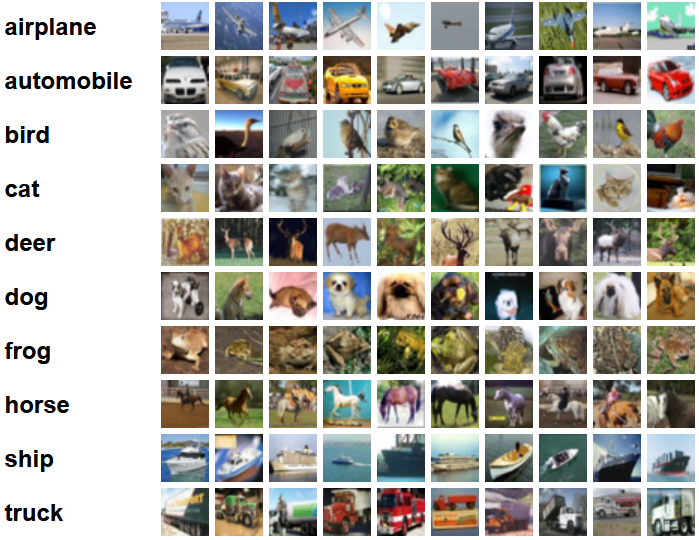
\includegraphics[width=0.6\textwidth]{MarcoTeorico/imgs/CIFAR-10.png}
    \caption{Dataset CIFAR-10.}
    \label{fig:cifar10}
\end{figure}

\subsubsection{Regresion}

Los problemas de regresión predicen un valor real. En otras palabras la función estima la variable dependiente conociendo la variable independiente.

La clase más común de regresión es la regresión lineal. La regresión lineal intenta llegar a una función que describa la relación entre $x$ y $y$, para valores conocidos de $x$, predice valores de $y$ que resultan ser precisos (\cite{patterson2017deep}).

\begin{figure}[H]
    \centering
    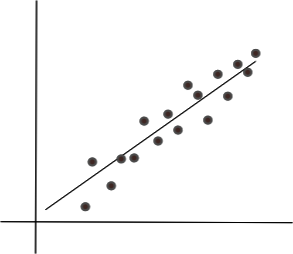
\includegraphics[width=0.5\textwidth]{MarcoTeorico/imgs/RegresionLineal.png}
    \caption{Grafica de regresión lineal.}
    \label{fig:regresionLineal}
\end{figure}

\subsection{Sobreajuste y Subajuste}

Cuando entrenamos un nuevo modelo buscamos que este tenga la capacidad de generalizar de tal manera que pueda interpretar datos de entrada que nunca haya visto.

Un buen modelo se equivoca poco en sus predicciones, esto significa que tiene un error bajo. Esto se evalúa ingresando al modelo datos que no recibió en su proceso de entrenamiento, de esta manera se tiene la seguridad de que el modelo es capaz de generalizar.

El subajuste ocurre cuando su modelo no puede obtener una pérdida suficientemente baja en el conjunto de entrenamiento. En este caso, su modelo no aprende los patrones en sus datos de entrenamiento. Por otro lado, tenemos un sobreajuste donde su red modela los datos de entrenamiento demasiado bien y no se generaliza a sus datos de validación (\cite{rosebrock2017deep}).


\begin{figure}[H]
    \centering
    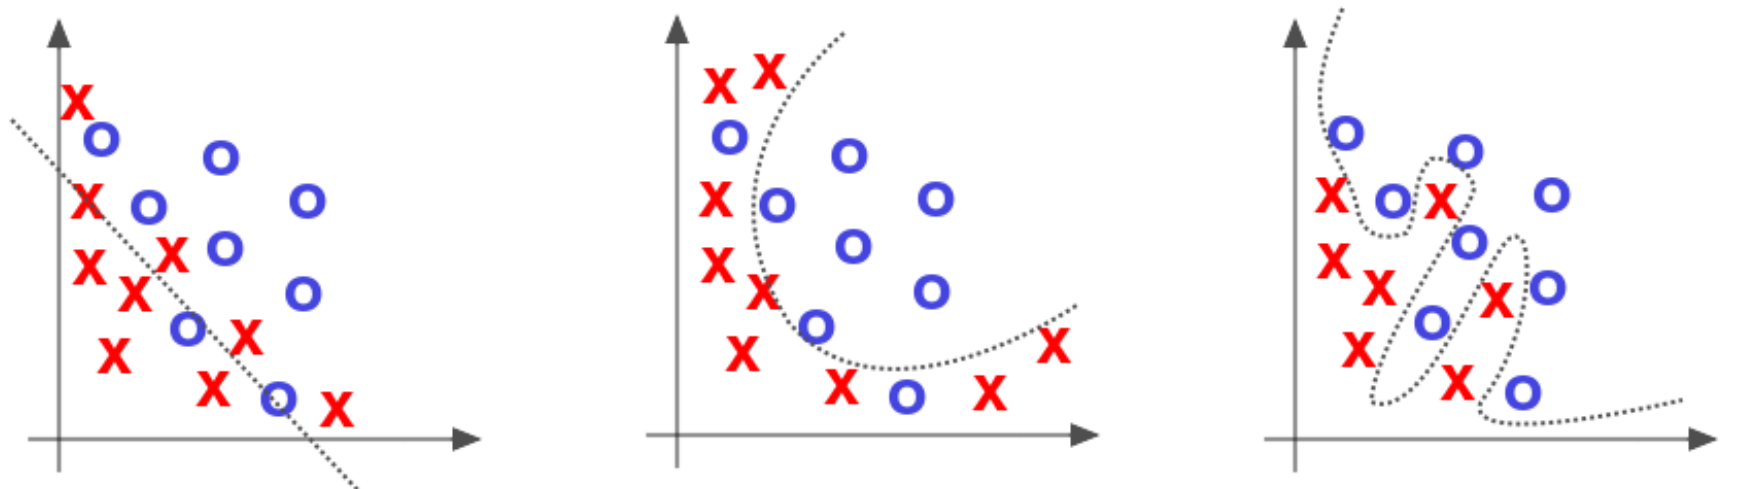
\includegraphics[width=0.8\textwidth]{MarcoTeorico/imgs/under-overfitting.png}
    \caption{Ejemplo de subajuste, ideal y sobreajuste.}
    \label{fig:underOverFtting}
\end{figure}
